% !TEX program = pdflatex
% 201909044006_蔡吉量_陈稼霖_李昌颖
\documentclass[12pt,a4paper]{article}
\linespread{1}
\usepackage{amsmath,amssymb,graphicx}
\usepackage[margin=1in]{geometry}
\usepackage[UTF8]{ctex}
\usepackage{titlesec}
\titleformat{\section}{\zihao{4}\heiti}{\zihao{4}\heiti\thesection}{14pt}{\centering}
\titleformat{\subsection}{\zihao{-4}\heiti}{\thesubsection}{12pt}{}
\titleformat{\subsubsection}{\zihao{-4}\heiti}{\thesubsubsection}{12pt}{}
\usepackage{palatino}
\begin{document}
\begin{center}
{\zihao{3}\heiti高压油管进出燃油工作策略设计}\\
~\\
{\zihao{4}\heiti摘要}
\end{center}

本文研究高压油管供油和喷油工作策略,利用四阶Runge-Kutta法求解管内燃油的流体连续性方程,得到管内燃油压强关于时间的函数,进而调节与供油和喷油相关的决策变量,以实现管内油压稳定在目标值或定时达到目标值的规划目标。

本文首先定义规划问题的目标函数 —— 管内油压与目标压强偏差值 $\Delta P$ 的方差 $\text{Var}(\Delta P)$,从而刻画管内油压对目标值的平均逼近程度。

在问题1中,对于稳定管内油压的要求,先确定燃油质量与压强之间的关系:用四次多项式拟合附件3中的燃油弹性模量随压强变化的数据,将得到的经验公式代入注1中的压强-密度微分方程,求出燃油压强关于密度的函数 $P(\rho)$,再结合密度公式建立管内燃油质量与压强的关系。然后,根据质量守恒定律列出管内燃油的流体连续性方程,将根据注2定义的单向阀流量函数 $F_{\text{in}}$和题设的喷油器流量函数 $F_{\text{out}}$ 代入连续性方程中,利用四阶Runge-Kutta方法计算油压偏差值关于时间的函数 $\Delta P(t)$,进而得到其方差$\text{Var}(\Delta P)$。最后,以供油单向阀的每次开启时长 $t_0$ 作为问题的决策变量,以最小化目标函数 $\text{Var}(\Delta P)$,得到最佳供油策略为单向阀每次开启时长 $t_0=0.288$ ms。

对于问题1中在规定时间达到目标油压的要求,注意到改变单向阀每次开启时长 $t_0$ 会造成管内燃油最终压强 $P_{\text{稳定}}$ 和达到最终油压 $T_{\text{稳定}}$ 所需时间同时变化,从而得出单向阀单次开启时间 $t_0$ 不随时间变化的方案无法满足要求的结论。据此,设计单向阀开启时长 $t_0$ 为一关于时间的分段函数,以该分段函数中的参数 $t_{01}$ 和 $T_{\text{转换}}$ 作为决策变量,管内油压达到目标油压所需时间与规定时间的偏差 $|T_{\text{稳定}}-T_{\text{规定}}|$ 和 管内实际油压基本稳定后与目标值偏差值的方差 $\text{Var}(P-150)$ 作为目标函数,进行多目标规划,从而得到新的供油策略。

在问题2中,以问题1中高压油泵内燃油的连续性方程为基础,与高压油泵内燃油的连续性方程联立为方程组,从驱动高压油泵的凸轮和控制喷油器出油的针阀的工作原理出发,根据注1中的流量函数计算新的供油和喷油流量函数,求解连续性方程组计算偏差值 $\Delta P(t)$ 及其方差 $\text{Var}(\Delta P)$。以凸轮角速度 $\omega$ 为决策变量,规划得到最佳供油策略为凸轮角速度 $\omega=0.024\text{rad}\cdot\text{ms}^{-1}$。

在问题3中,对于双喷油嘴的情形,更新问题2中的喷油流量函数为两个喷油嘴的流量函数 $2F_{\text{out}1}$,用如上方法计算目标函数 $\text{Var}(\Delta P)$ 以凸轮角速度 $\omega$ 为决策变量,规划得到最佳供油策略为凸轮角速度 $\omega=0.041\text{rad}\cdot\text{ms}^{-1}$。对于双喷油嘴加一个减压阀的情形,将盆友流量函数替换为 $2F_{\text{out}1}$ 和一个减压阀流量函数 $F_{\text{out}2}$ 之和,计算目标函数 $\text{Var}(\Delta P)$,保持 $\omega$ 与第一问相同,以 $P_t$ 作为决策变量,规划得到 $P_t=102$ MPa 为维持管内油压的最佳策略。

最后,对本模型忽略管内各处压强差等缺陷进行了分析和讨论。\\
~\\
关键词:质量守恒定律\quad流体连续性方程\quad Runge-Kutta方法\quad非线性规划
\newpage

\section{问题重述}

\subsection{问题背景}
燃油进入和喷出高压油管是许多燃油发动机工作的基础。图\ref{gaoyayouguanshiyitu}给出了某高压燃油系统的工作原理,燃油经过高压油泵从 A 处进入高压油管,再由喷口 B 喷出。燃油进入和喷出的间歇性工作过程会导致高压油管内压力的变化,使得所喷出的燃油量出现偏差,从而影响发动机的工作效率。
\begin{figure}[h]
\centering
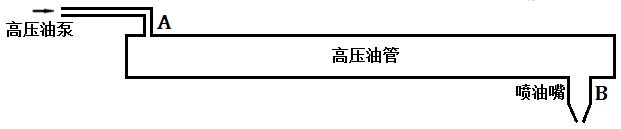
\includegraphics[scale=1]{gaoyayouguanshiyitu.jpg}
\caption{高压油管示意图}\label{gaoyayouguanshiyitu}
\end{figure}

\subsubsection{问题提出}
\textbf{\songti问题1.} 某型号高压油管的内腔长度为 $500$ mm,内直径为 $10$ mm,供油入口 A 处小孔的直径为 $1.4$mm,通过单向阀开关控制供油时间的长短,单向阀每打开一次后就要关闭 $10$ ms。喷油器每秒工作 $10$ 次,每次工作时喷油时间为 $2.4$ ms,喷油器工作时从喷油嘴 B 处向外喷油的速率如图\ref{penyousulvshiyitu}所示。高压油泵在入口 A 处提供的压力恒为 $160$ MPa,高压油管内的初始压力为 $100$ MPa。如果要将高压油管内的压力尽可能稳定在 $100$ MPa 左右,如何设置单向阀每次开启的时长?如果要将高压油管内的压力从$100$MPa 增加到$150$MPa,且分别经过约 $2$ s、$5$ s 和 $10$ s 的调整过程后稳定在 $150$MPa,单向阀开启的时长应如何调整?
\begin{figure}[h]
\centering
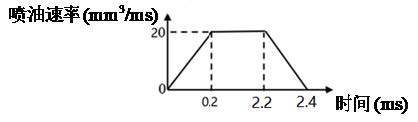
\includegraphics[scale=1]{penyousulvshiyitu.jpg}
\caption{喷油速率示意图}\label{penyousulvshiyitu}
\end{figure}

\textbf{\songti问题2.} 在实际工作过程中,高压油管 A 处的燃油来自高压油泵的柱塞腔出口,喷油由喷油嘴的针阀控制。高压油泵柱塞的压油过程如图\ref{gaoyayouguanshijigongzuoguochengshiyitu}所示,凸轮驱动柱塞上下运动,凸轮边缘曲线与角度的关系见附件1。柱塞向上运动时压缩柱塞腔内的燃油,当柱塞腔内的压力大于高压油管内的压力时,柱塞腔与高压油管连接的单向阀开启,燃油进入高压油管内。柱塞腔内直径为 $5$ mm,柱塞运动到上止点位置时,柱塞腔残余容积为 $20$ mm$^3$。柱塞运动到下止点时,低压燃油会充满柱塞腔(包括残余容积),低压燃油的压力为$0.5$MPa。喷油器喷嘴结构如图\ref{penyouqipenzuifangdahoudeshiyitu}所示,针阀直径为 $2.5$ mm、密封座是半角为$9^{\circ}$的圆锥,最下端喷孔的直径为 $1.4$ mm。针阀升程为 $0$ 时,针阀关闭;针阀升程大于 $0$ 时,针阀开启,燃油向喷孔流动,通过喷孔喷出。在一个喷油周期内针阀升程与时间的关系由附件2给出。在问题1中给出的喷油器工作次数、高压油管尺寸和初始压力下,确定凸轮的角速度,使得高压油管内的压力尽量稳定在 $100$ MPa 左右。
\begin{figure}[h]
\centering
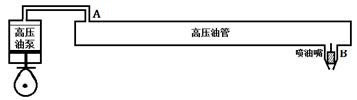
\includegraphics[scale=1]{gaoyayouguanshijigongzuoguochengshiyitu.jpg}
\caption{高压油管实际工作过程示意图}\label{gaoyayouguanshijigongzuoguochengshiyitu}
\end{figure}
\begin{figure}[h]
\centering
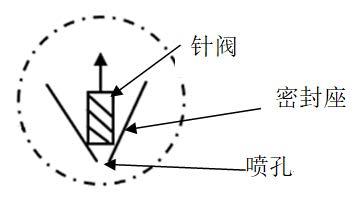
\includegraphics[scale=1]{penyouqipenzuifangdahoudeshiyitu.jpg}
\caption{喷油器喷嘴放大后的示意图}\label{penyouqipenzuifangdahoudeshiyitu}
\end{figure}

\textbf{\songti问题3.} 在问题2的基础上,再增加一个喷油嘴,每个喷嘴喷油规律相同,喷油和供油策略应如何调整?为了更有效地控制高压油管的压力,现计划在 D 处安装一个单向减压阀(图\ref{juyoujianyafahelianggepenyouzuishigaoyayouguanshiyitu})。单向减压阀出口为直径为 $1.4$ mm的圆,打开后高压油管内的燃油可以在压力下回流到外部低压油路中,从而使得高压油管内燃油的压力减小。请给出高压油泵和减压阀的控制方案。
\begin{figure}[h]
\centering
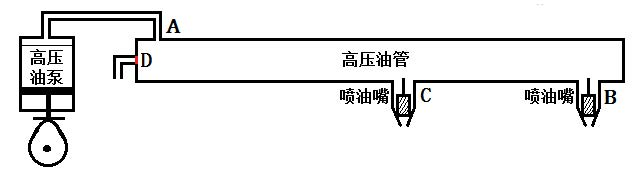
\includegraphics[scale=1]{juyoujianyafahelianggepenyouzuishigaoyayouguanshiyitu.jpg}
\caption{具有减压阀和两个喷油嘴时高压油管示意图}\label{juyoujianyafahelianggepenyouzuishigaoyayouguanshiyitu}
\end{figure}

\textbf{\songti注1.} 燃油的压力变化量与密度变化量成正比,比例系数为 $\frac{E}{\rho}$,其中 $\rho$ 为燃油的密度,当压力为 $100$ MPa时,燃油的密度为 $0.850$ mg/mm$^{3}$。$E$ 为弹性模量,其与压力的关系见附件3。

\textbf{\songti注2.} 进出高压油管的流量为 $Q=CA\sqrt{\frac{2\Delta P}{\rho}}$,其中 $Q$ 为单位时间流过小孔的燃油量(mm$^3$/ms),$C=0.85$ 为流量系数,$A$ 为小孔的面积(mm$^2$),$\Delta P$ 为小孔两边的压力差(MPa),$\rho$ 为高压侧燃油的密度(mg/mm3)。

\section{问题分析}

\subsection{规划目标分析}
题目要求通过调节供油和喷油策略,以使高压油管内的燃油压强尽可能稳定在某一目标值,或是在规定时间内达到某一目标值,其本质是一个规划问题。因此应当首先设置一个有关管内实际油压与目标压强偏差的目标函数,刻画管内实际油压逼近理想压强的程度。

\subsection{问题1第一问分析}
问题1中第一问要求设置单向阀每次开启时长以使管内油压稳定在 $100$ MPa,是一个单决策变量单目标的规划问题。首先根据质量守恒定律,列出管内燃油的流体连续性方程并求解得到管内油压关于时间的函数,进而计算油压与目标值偏差值的标准差。然后,以单向阀每次开启时长为决策变量,规划得到其使目标函数最小的最优值。

\subsection{问题1第二问分析}
问题1中第二问的要求是管内油压在规定时间内从初始值上升到 $150$ Mpa,管内燃油最终压强和达到这一压强所需的时间构成了规划问题的两个目标,改变单向阀每次开启时长会同时影响这两个变量的变化。因此,给定的单向阀开启时长很难同时实现两个目标,需要设计一个新的随时间变化的单向阀每次开启时长函数,并改变函数中相关参数进行规划。

\subsection{问题2分析}
在问题2中需要考虑高压油管供油和喷油的具体工作机制,因此需要以问题1中的连续性方程为基础,从凸轮和针阀的运动情况出发,根据注1中流量的参考公式计算新的供油和喷油流量函数,重新计算管内油压与目标偏差值的标准差。然后,以凸轮的角速度为决策变量,规划得到其使目标函数最小的最优值。

\subsection{问题3第一问分析}
问题3中第一问中增设一个喷油嘴,因此只需将问题2中的喷油流量函数更新为原来的 $2$ 倍,重复问题2的规划过程即可。

\subsection{问题3第二问分析}
问题3中第二问继续增设一个减压阀,因此需要在第一问的基础上相应地增设一个回流流量函数。以减压阀开启的阈值压强作为决策变量进行规划。

\section{模型假设}
\begin{itemize}
\item[1.] 题目提供的所有数据均真实可信;
\item[2.] 单向阀、喷油嘴、高压油泵及均能按照题目或本文设定的控制方案精确工作;
\item[3.] 高压油管的容积保持恒定而不随内部压力发生变化;
\item[4.] 在本文所考虑的压力范围内,燃油为可任意压缩的流体,燃油永远填充满高压油管,即管内燃油体积恒等于油管容积;
\item[5.] 燃油压缩时的温度变化可忽略;
\item[6.] 油管内燃油密度、压强等参数处处均匀。
\end{itemize}
\section{符号说明与名词解释}
\subsection{符号说明}
\begin{table}[h]
\centering
\begin{tabular}{cp{10cm}}

符号 & 符号含义\\\hline
$m$ & 高压油管中的油量的变化量\\
$m_h$ & 高压油泵内燃油质量\\
$V$ & 油管的容积\\
$\rho$ & 油管内燃油密度\\
$\rho_h$ & 油泵内燃油密度\\
$P$ & 管内油压\\
$P_h$ & 油泵内燃油压强\\
$F_{\text{in}}$ & 油从油泵流入油管的燃油质量\\
$F_{\text{out}}$ & 油从油管流出的质量\\
$F_{\text{out}2}$ & 单位时间内由减压阀流出燃油质量\\
$Q_{\text{in}}$ & 单位时间内从油泵流入油管的燃油体积\\
$Q_{\text{out}}$ & 单位时间内从油管流出的燃油体积\\
\end{tabular}
\end{table}
本文中,若无特别说明,质量单位统一采用毫克(mg),长度单位统一采用毫米(mm),时间单位统一采用毫秒(mm),压强单位统一采用兆帕(MPa),角度统一采用弧度制。

\section{模型建立和求解}
\subsection{规划目标函数设定}
首先,定义规划问题的目标函数。虽然题目的要求是保证管内油压尽可能稳定在目标压强,但由于单向阀与喷油器的工作方式均为间歇式的,因此在大部分时间段管内实际油压与目标压强间存在随时间改变的偏差
\begin{equation}
\Delta P(t)=P(t)-P_0
\end{equation}
其中 $P(t)$ 为 $t$ 时刻管内油压,$P_0$ 为题设给定的目标压强。

定义这一偏差值的方差
\begin{equation}
\label{Var}
\text{Var}(\Delta P)=\frac{1}{T}\int_0^T\Delta P^2(t)dt
\end{equation}
为目标函数。当给定足够大的积分上限 $T$ 时,$\text{Var}(\Delta P)$ 越小,则表明压强越稳定且越逼近目标值,因此 $Var(\Delta P)$ 可以较好地刻画实际压强与目标值间的平均偏差情况。

\subsection{问题1第一问求解:设定单项阀每次开启时长以维持油压稳定}
由于管内燃油膨胀和收缩以使自身体积始终等于高压油管体积,因此在高压油管工作过程中,燃油体积并非一守恒量而为燃油质量。根据质量守恒定律,油管内燃油的质量改变量等于进入油管的燃油质量与喷出油管的燃油质量之差,即燃油的流体连续性方程
\begin{equation}
\label{cntequ}
\Delta m(T)=\int_0^TF_{\text{in}}(t)dt-\int_0^TF_{\text{out}}(t)dt
\end{equation}
其中 $\Delta m$ 为给定时间段 $T$ 内高压油管内燃油的质量改变量,$F_{\text{in}}(t)$ 和 $F_{\text{out}}(t)$ 分别在单位时间内进入和喷出高压油管的燃油质量。

为便于求解,将该流体连续性方程改写为微分形式
\begin{equation}
\label{cntequ2}
\frac{\text{d}(\Delta m)}{\text{d} t}=F_{\text{in}}(t)-F_{\text{out}}(t)
\end{equation}

下面对式(\ref{cntequ2})中各项进行建模并求解。

\textbf{\songti STEP 1} 式(\ref{cntequ2})两端均为关于燃油质量的函数,然而问题的目标函数却是关于管内燃油压强的函数,因此首先应当建立管内燃油质量与压强之间的关系。根据注1,燃油的压力变化量与密度变化量之比为$\frac{E}{\rho}$,由此可以列出微分方程
\begin{equation}
\label{P-rho}
\frac{\text{d}P}{\text{d}\rho}=\frac{E}{\rho}
\end{equation}
其中 $\rho$ 为燃油的密度,$E$ 为燃油的弹性模量,它是关于燃油压强的函数。

% 根据最小二乘法原理,用4次多项式拟合附件3中的数据(MATLAB代码见附件"Problem\_1\_E\_rho.m"),得到燃油弹性模量关于压强的经验公式
根据附件3中的数据,燃油的弹性模量 $E$ 随着压强的增大而单调递增。使用 MATLAB 中的 curve fitting 工具箱对附件3中的数据做4次多项式拟合,得到燃油弹性模量关于压强的经验公式
\begin{equation}
\label{E-P}
E(P)=a_1P^4+b_1P^3+c_1P^2+d_1P+e_1
\end{equation}
其中各项系数 $a_1=3.454\times10^{-7}$,$b_1=-3.813\times10^{-5}$,$c_1=0.01667$,$d_1=4.688$,$e_1=1540$,拟合优度 $R^2=0.999999$,均方根误差为 $0.4754$,数据点和拟合曲线见图。
\begin{figure}[h]
\centering
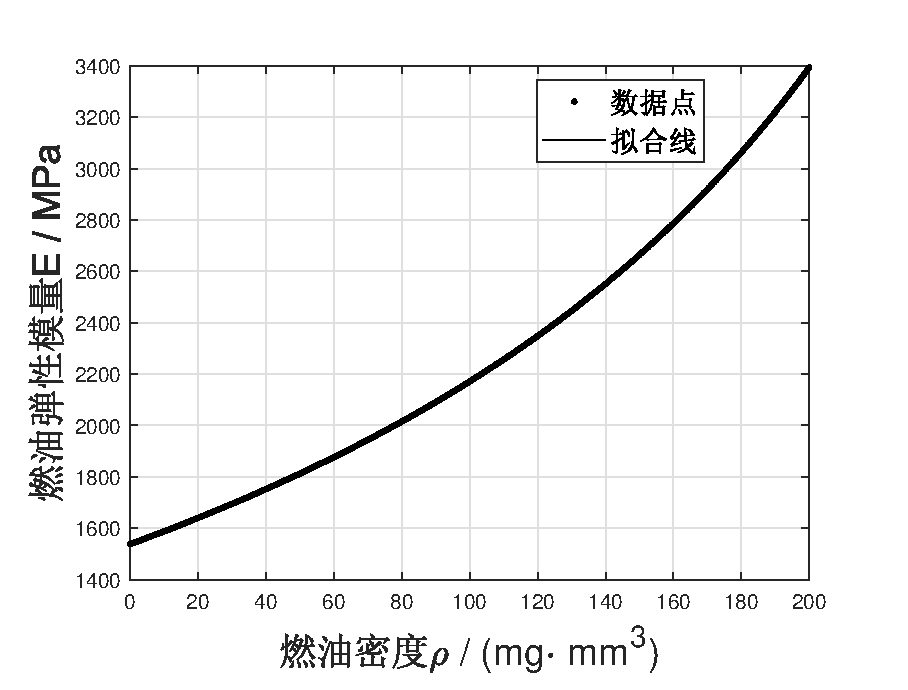
\includegraphics[scale=0.75]{Problem_1_E_rho.eps}
\caption{燃油弹性模量关于压强的经验公式}\label{Problem_1_E_r}
\end{figure}

将得到的经验公式(\ref{E-P})代回微分方程(\ref{P-rho})中,利用四阶Runge-Kutta方法求解出 $\rho$ 关于 $P$ 的数值解,并用最小二乘法拟合得到 $\rho$ 关于 $P$ 的2次多项式型函数
\begin{equation}
\label{rho-P}
\rho=f(P)=a_2P^2+b_2P+c_2
\end{equation}
其中各项系数 $a_2=-6.570\times10^{-7}$,$b_2=5.230\times10^{-4}$,$c_2= 0.8043$,拟合优度 $R^2=*$,均方根误差 $0.4754$。
% 需要拟合优度!

取式(\ref{rho-P})反函数还可以 $P$ 关于 $\rho$ 的函数
\begin{equation}
\label{P-rho2}
P=\frac{-b_2+\sqrt{b_2^2-4a_2(c_2-\rho)}}{2a_2}
\end{equation}

油管内燃油质量可由
\begin{equation}
\label{rho}
m=\rho V
\end{equation}
计算,其中高压油管的容积为
\begin{equation}
\label{volumn}
V=\pi\left(\frac{D}{2}\right)^2L=\pi\times\left(\frac{10}{2}\right)^2\times500\text{ mm}^3=12500\pi\text{ mm}^3
\end{equation}
从而式(\ref{cntequ2})左端可以表示为
\begin{equation}
\frac{\text{d}(\Delta m)}{\text{d}t}=\frac{\text{d}(\rho V)}{\text{d}t}=V\frac{\text{d}\rho}{\text{d}t}=V\frac{\text{d}\rho}{\text{d}P}\frac{\text{d}P}{\text{d}t}=V\frac{\rho}{E}\frac{\text{d}P}{\text{d}t}
\end{equation}
其中 $\rho$ 为高压油管中燃油的密度。将式(\ref{E-P})和式(\ref{rho-P})代入上式可以得到 $\frac{\text{d}(\Delta m)}{\text{d}t}$ 关于 $P$ 的函数
\begin{equation}
\label{dmdt-P}
\frac{\text{d}(\Delta m)}{\text{d}t}=V\frac{a_2P^2+b_2P+c_2}{a_1P^4+b_1P^3+c_1P^2+d_1P+e_1}\frac{\text{d}P}{\text{d}t}
\end{equation}

\textbf{\songti STEP 2} 然后再来分别确定 $F_{\text{in}}$ 和 $F_{\text{out}}$。

对于 $F_{\text{in}}$,
\begin{equation}
\label{Fin}
F_{\text{in}}(t)=\rho_hQ_{\text{in}}(t)
\end{equation}
其中 $\rho_h$ 为来自高压油泵($160$ MPa)的燃油密度,根据式(\ref{rho-P})计算得 $\rho_h=f(160)=0.8711\text{ mg}/\text{mm}^3$,$Q_{\text{in}}$ 为单位时间内进入高压油管的燃油体积,根据单向阀每打开一次后就要关闭 $10$ ms 的题设和注2,$Q_{\text{in}}(t)$ 具有 $(t_0+10)$ ms 的周期,且在它的一个周期 $[0,t_0+10)$ ms 中有
\begin{equation}
\label{Qin}
Q_{\text{in}}(t)=\left\{\begin{array}{ll}
CA_{\text{in}}\sqrt{\frac{2(P_h-P)}{\rho_h}},&0\leq t\leq t_0\\
0,&t_0<t<t_0+10
\end{array}\right.
\end{equation}
其中 $t$ 为每次 $C=0.85$ 为流量系数,$A_{\text{in}}=\pi(\frac{D_{\text{in}}}{2})^2=\pi(\frac{1.4}{2})^2\text{ mm}^2=0.49\pi\text{ mm}^2$为 A 处供油口截面积,$P_h=160$ MPa 为高压油泵在入口 A 处提供的压强。

利用 $Q_{\text{in}}$ 的周期性
\begin{equation}
Q_{\text{in}}(t+t_0+10)=Q_{\text{in}}(t)
\end{equation}
可将式(\ref{Qin})延拓到区间 $[0,+\infty)$。为了方便在计算机程序中表示和计算 $Q_{\text{in}}$ 又可改写为
\begin{equation}
\label{Qin2}
Q_{\text{in}}=CA\sqrt{\frac{2(P_h-P)}{\rho_h}}\cdot\left\{1-u[(t~~\text{mod}~~t_0+10)-t_0]\right\}
\end{equation}
其中 $u(x)$ 为单位阶跃函数,$(t~~\text{mod}~~t_0+10)$ 代表 $t$ 对 $t_1+10$ 取模得到的余数。

\textbf{\songti STEP 3} 对于 $F_{\text{out}}$,
\begin{equation}
\label{Fout}
F_{\text{out}}=\rho Q_{\text{out}}(t)
\end{equation}
其中 $\rho$ 为管内燃油密度,根据式(\ref{rho-P})可以表达为关于 $P$ 的函数,$Q_{\text{in}}$ 为单位时间内喷出高压油管的燃油体积,根据题设,$Q_{\text{out}}$ 亦为周期函数,喷油口工作周期为 $100$ ms ,根据图\ref{penyousulvshiyitu}知,在其一个周期 $[0,10)$ ms 中有
\begin{equation}
Q_{\text{out}}(t)=\left\{\begin{array}{ll}
\frac{20}{0.2}t,&0\leq t<0.2\\
20,&0.2\leq t<2.2\\
-\frac{20}{0.2}(t-2.4),&2.2\leq t<2.4\\
0,&2.2\leq t<10-2.4
\end{array}\right.
\end{equation}
同理根据周期性可以写出适合计算机处理的 $Q_{\text{out}}(t)$
\begin{align}
\nonumber Q_{\text{out}}(t)=&100t\\
\nonumber&-100[(t~~\text{mod}~~10)-0.2]\cdot u[(t~~\text{mod}~~10)-0.2]\\
\nonumber&-100[(t~~\text{mod}~~10)-2.2]\cdot u[(t~~\text{mod}~~10)-2.2]\\
\label{Qout}&+100[(t~~\text{mod}~~10)-2.4]\cdot u[(t~~\text{mod}~~10)-2.4]
\end{align}

\textbf{\songti STEP 4} 将式(\ref{dmdt-P}),(\ref{Fin}),(\ref{Qin2}),(\ref{Fout})和(\ref{Qout})代入式(\ref{cntequ2})中,利用Runge-Kutta方法求解出不同 $t_0$ 下管内油压的变化情况 $P(t)$ 并根据式(\ref{Var})计算不同 $t_0$ 对应的目标函数 $\text{Var}(\Delta P)$(MATLAB见附件“Problem\_1\_1.m”),如图\ref{Problem_1_1}。
\begin{figure}[h]
\centering
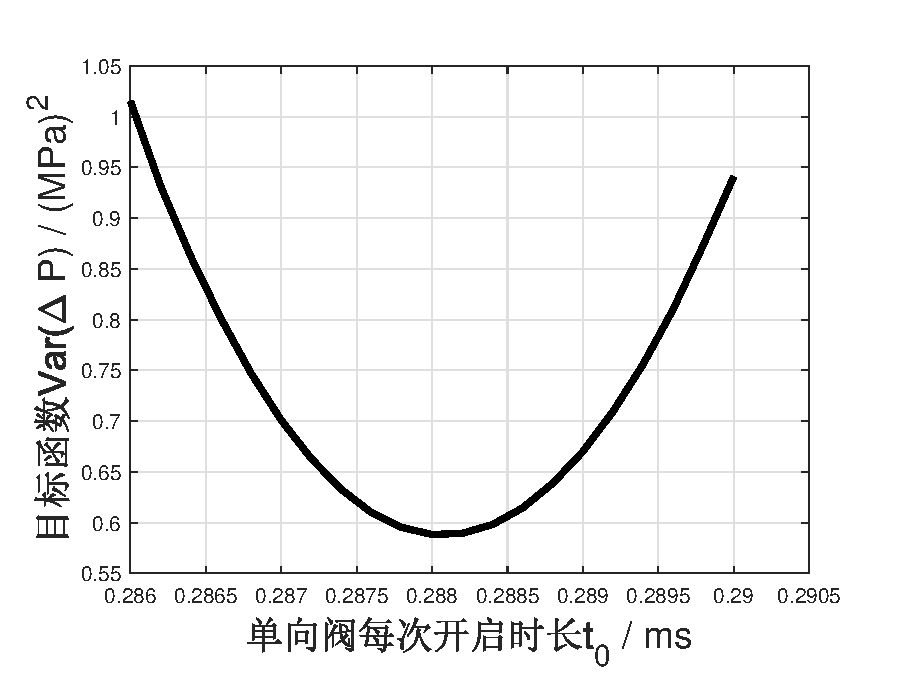
\includegraphics[scale=0.75]{Problem_1_1.eps}
\caption{目标函数与单向阀每次开启时长关系图}\label{Problem_1_1}
\end{figure}

根据计算结果,目标函数随着 $t_0$ 的增大先递增后递减,最小点为 $t_0=0.288$ ms,此即使管内燃油压强稳定在 $100$ MPa 的单向阀每次开启时长 $t_0$ 的最佳值。

\subsection{问题1第二问求解:使管内油压定时达到目标值}
问题1第二问中包含两个目标,一是管内油压基本稳定时逼近目标值 $150$ MPa,二是需要在规定的时间达到这一目标值,然而利用上小结中的方法进行模拟时,若每次模拟给定单向阀开启时长 $t_0$,则在本文所讨论的范围内管内油压最终稳定值 $P_{\text{稳定}}$ 随着 $t_0$递增(如图\ref{P_stable-t_0},代码见附件“Problem\_1\_2\_1.m”),而达到稳定值所需的时间 $T_{\text{稳定}}$ 则随着 $t_0$无规则波动(如图\ref{T_stable-t_0},代码见附件“Problem\_1\_2\_1.m”),无法同时实现两个规划目标。因此,需要设计 $t_0$ 随管内油压变化的工作策略。
\begin{figure}[htbp]
\centering
\begin{minipage}[t]{0.48\textwidth}
\centering
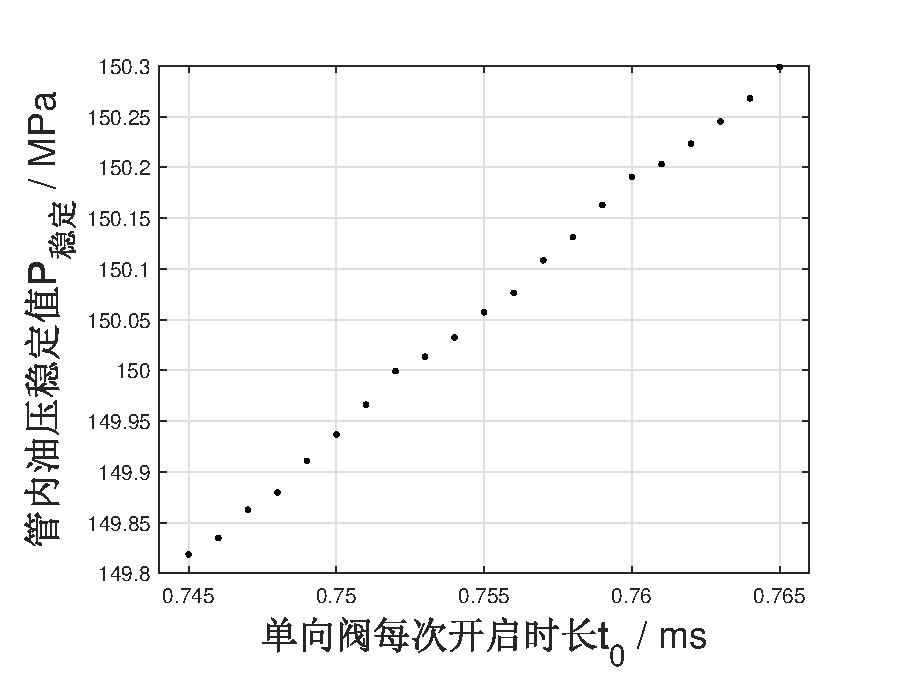
\includegraphics[width=7.5cm]{Problem_1_2_P_stable-t_0.eps}
\caption{管内油压最终稳定值随单向阀每次开启时长变化关系}\label{P_stable-t_0}
\end{minipage}
\begin{minipage}[t]{0.48\textwidth}
\centering
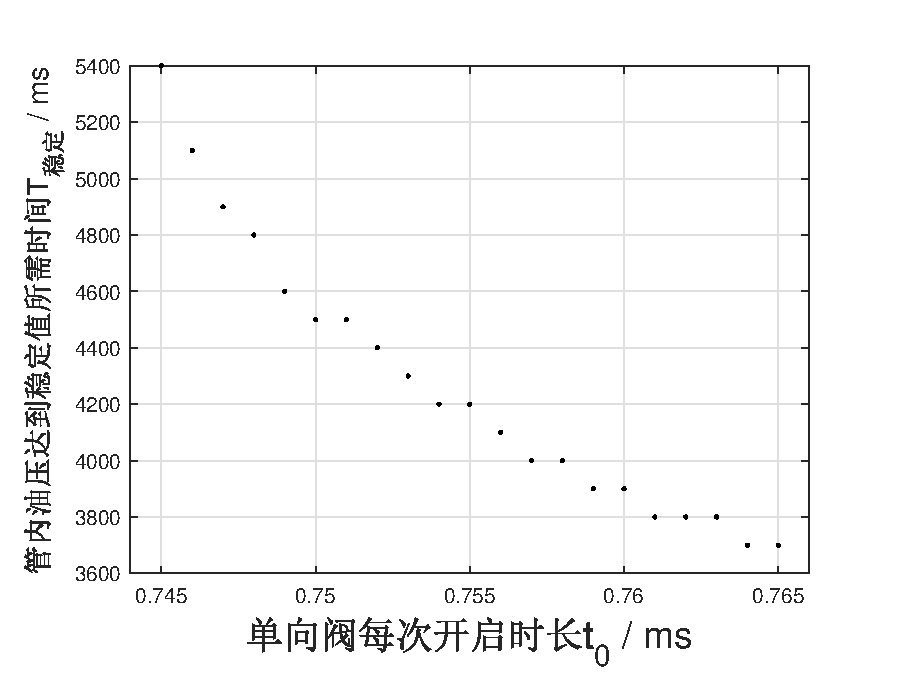
\includegraphics[width=7.5cm]{Problem_1_2_T_stable-t_0.eps}
\caption{管内油压达到目标值所需时间随单向阀每次开启时长变化关系}\label{T_stable-t_0}
\end{minipage}
\end{figure}

由图\ref{P_stable-t_0},可知管内油压最终基本稳定在 $150$ MPa,需要 $t_0=0.752$ ms,但若在整个工作中保持 $t_0=0.752$ ms,则管内油压将在约 $4400$ ms达到目标值,因此,设计单向阀每次开启时间随压强变化的函数为一分段函数,在初始一段时间内以较小(或较大)的每次开启时长 $t_{01}$ 工作,在后面一段时间内以 $0.752$ ms 的每次开启时长工作
\begin{equation}
t_0(t)=\left\{\begin{array}{ll}
t_{01},&0\leq t<T_{\text{转换}}\\
0.752,&t\geq T_{\text{转换}}
\end{array}\right.
\end{equation}
其中 $T_{\text{转换}}$ 为两种每次开启时长工作方式转换的时间节点。

以 $t_{01}$ 和转换时间 $T_{\text{转换}}$ 为决策变量,以达到目标压强的时间与规定时间的差值 $|T_{\text{稳定}}-T_{\text{规定}}|$ 和管内实际油压基本稳定后与目标值偏差值的方差 $\text{Var}(P-150)|_{t>T_{\text{规定}}}$ 为目标函数,调节决策变量来在两个目标函数中的前者小于阈值 $\varepsilon=10^{-1}$ ms 的情况下,取后者的最小值(MATLAB代码见附件“Problem\_1\_2\_2.m”)。
\begin{align}
&\min\quad\text{Var}(P-150)|_{t>T_{\text{规定}}}\\
&\left\{\begin{array}{l}
t_{01}>0\\
t_{01}\left\{\begin{array}{ll}<0.752,&\text{若 }T_{\text{规定}}\leq13900\\>0.752,&\text{若 }T_{\text{规定}}>13900\end{array}\right.\\
0<T_{\text{转换}}<T_{\text{规定}}\\
|T_{\text{稳定}}-T_{\text{规定}}|<\varepsilon
\end{array}\right.
\end{align}

由此,得到
\begin{itemize}
\item[1.] 对于 $T_{\text{规定}}=2000$ ms,应取 $t_{01}=0.900$,$T_{\text{转换}}=1750$ ms,模拟得到管内油压变化曲线如图\ref{Problem_1_2_P_t_2s};
\item[2.] 对于 $T_{\text{规定}}=5000$ ms,应取 $t_{01}=0.600$,$T_{\text{转换}}=1360$ ms,模拟得到管内油压变化曲线如图\ref{Problem_1_2_P_t_2s};
\item[3.] 对于 $T_{\text{规定}}=10000$ ms,应取 $t_{01}=0.300$,$T_{\text{转换}}=5610$ ms,模拟得到管内油压变化曲线如图\ref{Problem_1_2_P_t_2s}。
\end{itemize}
\begin{figure}[htbp]
\centering
\begin{minipage}[t]{0.48\textwidth}
\centering
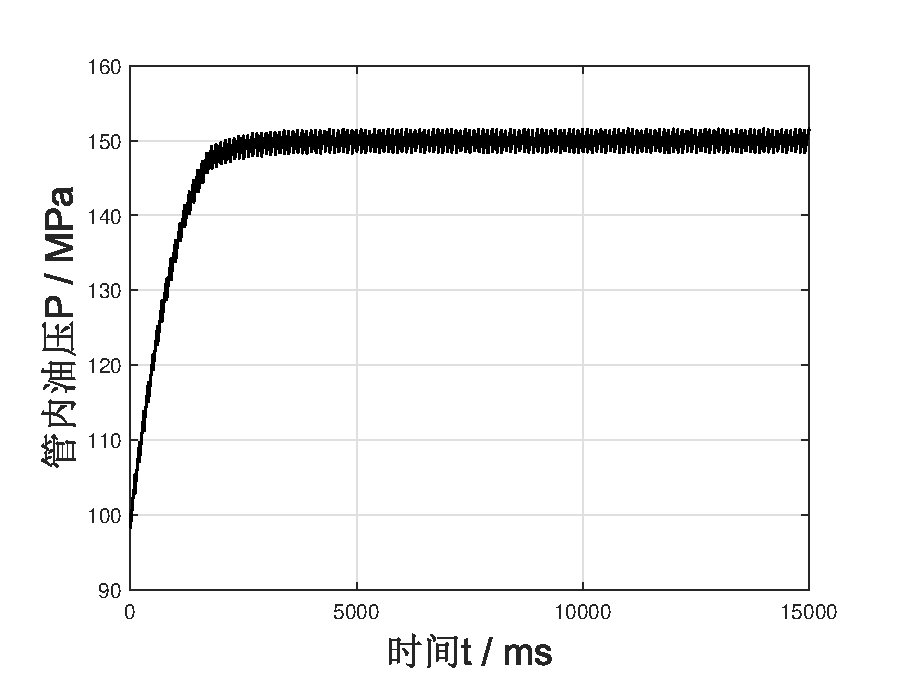
\includegraphics[width=7.5cm]{Problem_1_2_P_t_2s.eps}
\caption{$T_{\text{规定}}=2000$ s时单向阀最佳工作略下管内油压随时间变化情况}\label{Problem_1_2_P_t_2s}
\end{minipage}
\begin{minipage}[t]{0.48\textwidth}
\centering
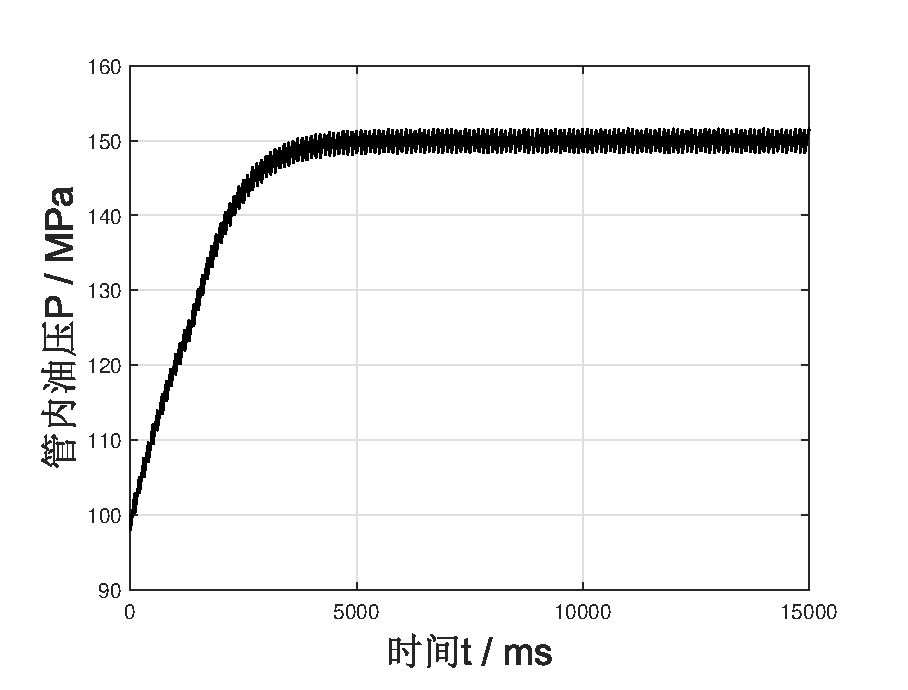
\includegraphics[width=7.5cm]{Problem_1_2_P_t_5s.eps}
\caption{$T_{\text{规定}}=5000$ s时单向阀最佳工作略下管内油压随时间变化情况}\label{Problem_1_2_P_t_5s}
\end{minipage}
\begin{minipage}[t]{0.48\textwidth}
\centering
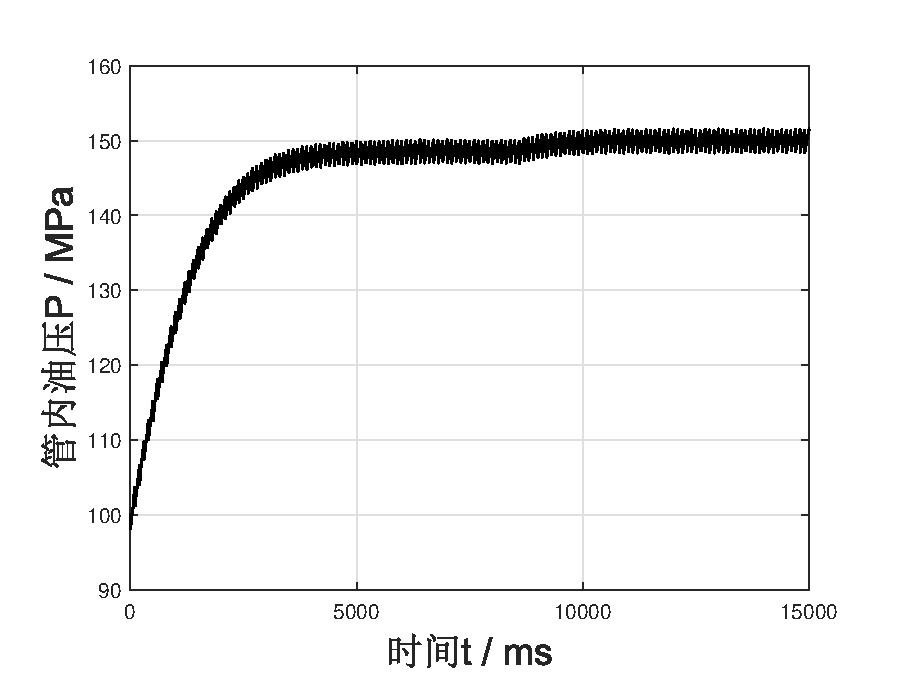
\includegraphics[width=7.5cm]{Problem_1_2_P_t_10s.eps}
\caption{$T_{\text{规定}}=10000$ s时单向阀最佳工作略下管内油压随时间变化情况}\label{Problem_1_2_P_t_10s}
\end{minipage}
\end{figure}

\subsection{问题2求解:设定凸轮角速度以维持油压稳定}
在问题2中在原有高压油管的基础上新增了一个容器--高压油泵,因此列出高压油泵中燃油在一个工作周期中的流体连续性方程
\begin{equation}
\label{cntequ_h}
\frac{\text{d}(\Delta m_h)}{\text{d}t}=-\int_0^TF_{\text{in}}dt
\end{equation}
其中 $\Delta m_h$ 为高压油泵中的燃油质量

高压油泵由凸轮驱动,而喷油器由针阀控制,因此需要分别根据这两者的运动状态重新确定 $F_{\text{in}}$ 和 $F_{\text{out}}$ 后再来求解连续性方程并对凸轮角速度 $\omega$ 进行规划。

\textbf{\songti STEP 1} 重新确定 $F_{\text{in}}$。

\textbf{\songti STEP 1.1} 由于单向阀的开合和流量与高压油泵内的压强有关,且高压油泵处于周期性的运转中。因此需要求解油泵内的流体连续性方程
\begin{equation}
\frac{\text{d}m_h}{\text{d}t}=-F_{\text{in}}
\end{equation}
得到油泵在一个工作周期(凸轮转一周)内的燃油压强变化情况,其中 $m_h$ 为油泵内燃油质量,$F_{\text{in}}$ 即为单位时间内有油泵流入油管的燃油质量,表示为
\begin{equation}
\label{cntequ3}
F_{\text{in}}=CA_{\text{in}}\sqrt{\frac{2(P_h-P)}{\rho_h}}u(P_h-P)
\end{equation}
其中流量系数 $C$ 和 A 处供油口截面积 $A_{\text{in}}$ 和第1题相同,下面对 $m_h$ 的初始值 $m_h(0)$,$\rho_h$ 和 $P$ 分别做具体讨论

\textbf{\songti STEP 1.2} 确定初始值 $m_h(0)$。

首先,需要对于凸轮的几何形貌有一个数学上的表示,故用三角函数拟合附件1中凸轮极径与极角的数据得到(MATLAB代码见附件“Problem\_2\_r\_theta.m”,数据点和拟合曲线如图\ref{Problem_2_r_theta})
\begin{equation}
r=a_3\cos(b_3\theta)+c_3
\end{equation}
其中 $r$ 为凸轮极径,$\theta$ 为凸轮极角,参数 $a_3=4.816$,$b_3=1.000$,$c_3=2.413$,拟合优度 $R^2=0.9999999997$,均方根误差为 $2.866\times10^{-5}$。
\begin{figure}[h]
\centering
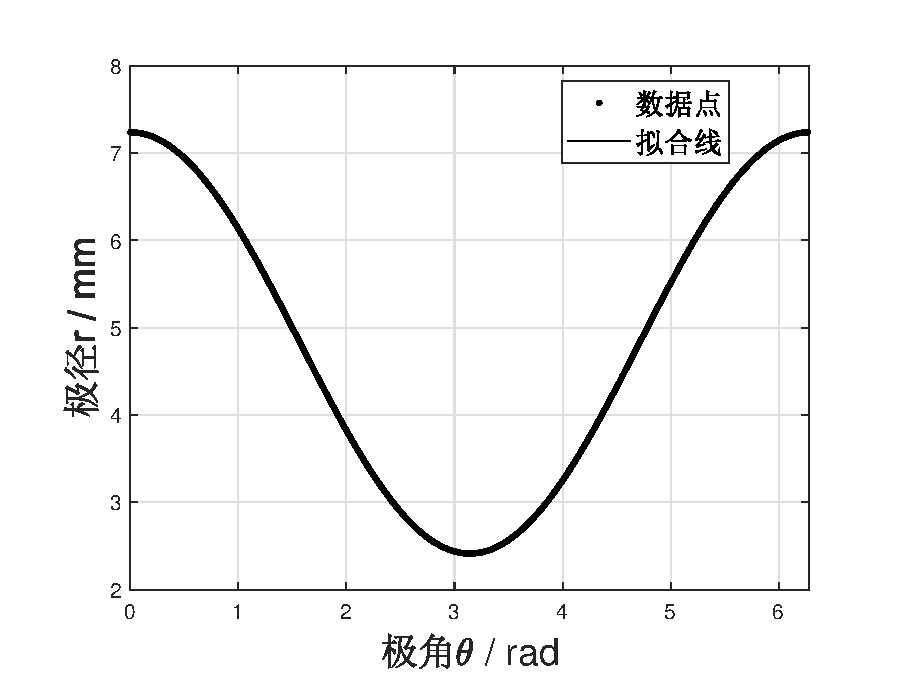
\includegraphics[scale=0.5]{Problem_2_r_theta.eps}
\caption{凸轮极径与极角关系拟合图}\label{Problem_2_r_theta}
\end{figure}

假设柱塞在 $t=0$ 时刻从最低点开始向上运动,则 $t$ 时刻柱塞与其路径最高点的距离为
\begin{equation}
\label{y-t}
y(t)=(a_3+c_3)-(a_3\cos(b_3\theta+\frac{\pi}{2})+c_3)=a_3[1+\sin(b_3\omega t)]
\end{equation}
此时,柱塞腔内容积为
\begin{equation}
V_h(t)=V_0+\pi(\frac{D_h}{2})^2y(t)
\end{equation}
其中 $V_0=20\text{ mm}^3$ 为柱塞腔残余容积,$D_h=5$ mm 为柱塞腔内直径,代入式(\ref{y-t})有
\begin{equation}
\label{Vh_t}
V_h(t)=20+30.1(1+\sin\omega t)
\end{equation}
$t=0$ 时刻柱塞腔内压强为 $0.5$ MPa,利用式(\ref{rho-P})得柱塞腔内初始燃油密度为 $f(0.5)=0.8046\text{ mg}/\text{mm}^3$,初始质量为
\begin{equation}
m_h(0)=\rho V_h(0)=76.21\text{mg}
\end{equation}

\textbf{\songti STEP 1.3} 表示泵内燃油密度 $\rho_h$ 的变化情况。

泵内燃油密度 $\rho_h$ 公式为
\begin{equation}
\label{rhoh_t}
\rho_h(t)=\frac{m_h}{V_h(t)}
\end{equation}

\textbf{\songti STEP 1.4} 关于管内油压 $P$ 的讨论。

由于油泵内燃油最大体积 $V_h=30.1563\pi\text{ mm}^3$ 远小于油管的容积 $V=12500\pi\text{ mm}^3$,且题目也要求规划结果保证管内油压稳定在 $100$ MPa,因此在\textbf{\songti STEP 1} 计算 $P_{h}$ 的过程中忽略由油泵进入油管内的燃油造成的管内油压变化,式(\ref{cntequ3})直接写作
\begin{equation}
\label{cntequ4}
F_{\text{in}}=CA_{\text{in}}\sqrt{\frac{2(P_h-100)}{\rho_h}}u(P_h-100)
\end{equation}

\textbf{\songti STEP 1.5} 将式(\ref{rhoh_t}) 代入式(\ref{cntequ4}),并用利用四阶Runge-Kutta方法求解得到 $m_h(t)$ 在油泵一个工作周期中的变化情况,回代入式(\ref{cntequ4})从而获得关于凸轮转速 $\omega$ 的一周期内由油泵进入油管的燃油流量函数 $F_{\text{in}}$ 的函数(无解析形式,但对给定 $\omega$ 有数值解)。

\textbf{\songti STEP 2.} 重新确定 $F_{\text{out}}$。

\begin{equation}
\label{Fout3}
F_{\text{out}}=CA_{\text{out}}\sqrt{\frac{2(P-P_{\text{大气}})}{\rho}}
\end{equation}
其中 $A_{\text{out}}$ 为由针阀控制的喷油嘴通道的有效截面,下面再做具体讨论,$P_{\text{大气}}=0.1$ MPa 为大气压强,$\rho=\frac{m}{V}$ 为管内燃油密度。

要确定 $A_{\text{out}}$ 根据附件2中的针阀运动数据,拟合得到其一个工作周期中升程的变化情况,如图\ref{needle}。
\begin{equation}
\label{x-t}
x=\left\{\begin{array}{ll}
 -772.34x^5+570.2x^4-96.50x^3+8.824x^2-0.2908&0\leq x<0.45\\
2&0.45\leq t<2\\
799.5x^5-9194x^4+42221x^3-96759x^2+110643x-50490&2\leq t<2.45
\end{array}\right.
\end{equation}
\begin{figure}[h]
\centering
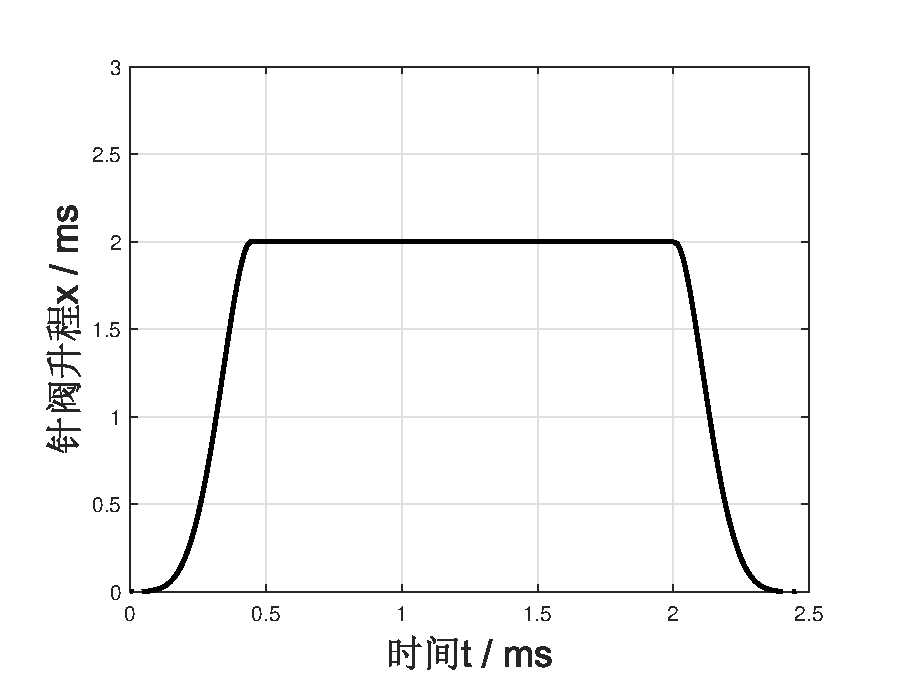
\includegraphics[scale=0.75]{needle.eps}
\caption{针阀升程随时间变化}\label{needle}
\end{figure}

由于喷射出的燃油流量受到喷油嘴最窄处限制,因此有效截面也表示为升程的分段函数
\begin{equation}
\label{Ain}
A_{\text{in}}=\left\{\begin{array}{ll}
\pi \tan^29^{\circ}(\frac{\sqrt{d_1^2+d_0^2}-d_1}{2\tan 9^{\circ}})^2+2\pi\tan 9^{\circ}\cdot\frac{\sqrt{d_1^2+d_0^2}-d_1}{2\tan 9^{\circ}}\frac{d_1}{2},&0\leq H\leq \frac{\sqrt{d_1^2+d_0^2}-d_1}{2\tan 9^{\circ}}\\
\pi(\frac{d_0}{2}),&x>\frac{\sqrt{d_1^2+d_0^2}-d_1}{2\tan 9^{\circ}}
\end{array}\right.
\end{equation}
其中 $d_1=2.5$ mm 为针阀的直径,$d_0=1.4$ mm为喷孔直径。

将式(\ref{Fout3}),(\ref{x-t}),(\ref{Ain})及 $F_{\text{in}}$ 代入流动性方程中结合式\ref{Var}求解得 $\text{Var}(\Delta P)$,以凸轮转动角速度 $\omega$为决策变量,规划得最佳值为 $\omega=0.024\text{ rad}/\text{ms}$(如图\ref{Problem_2},MATLAB代码见附件“Problem\_2.m”)。
\begin{figure}[h]
\centering
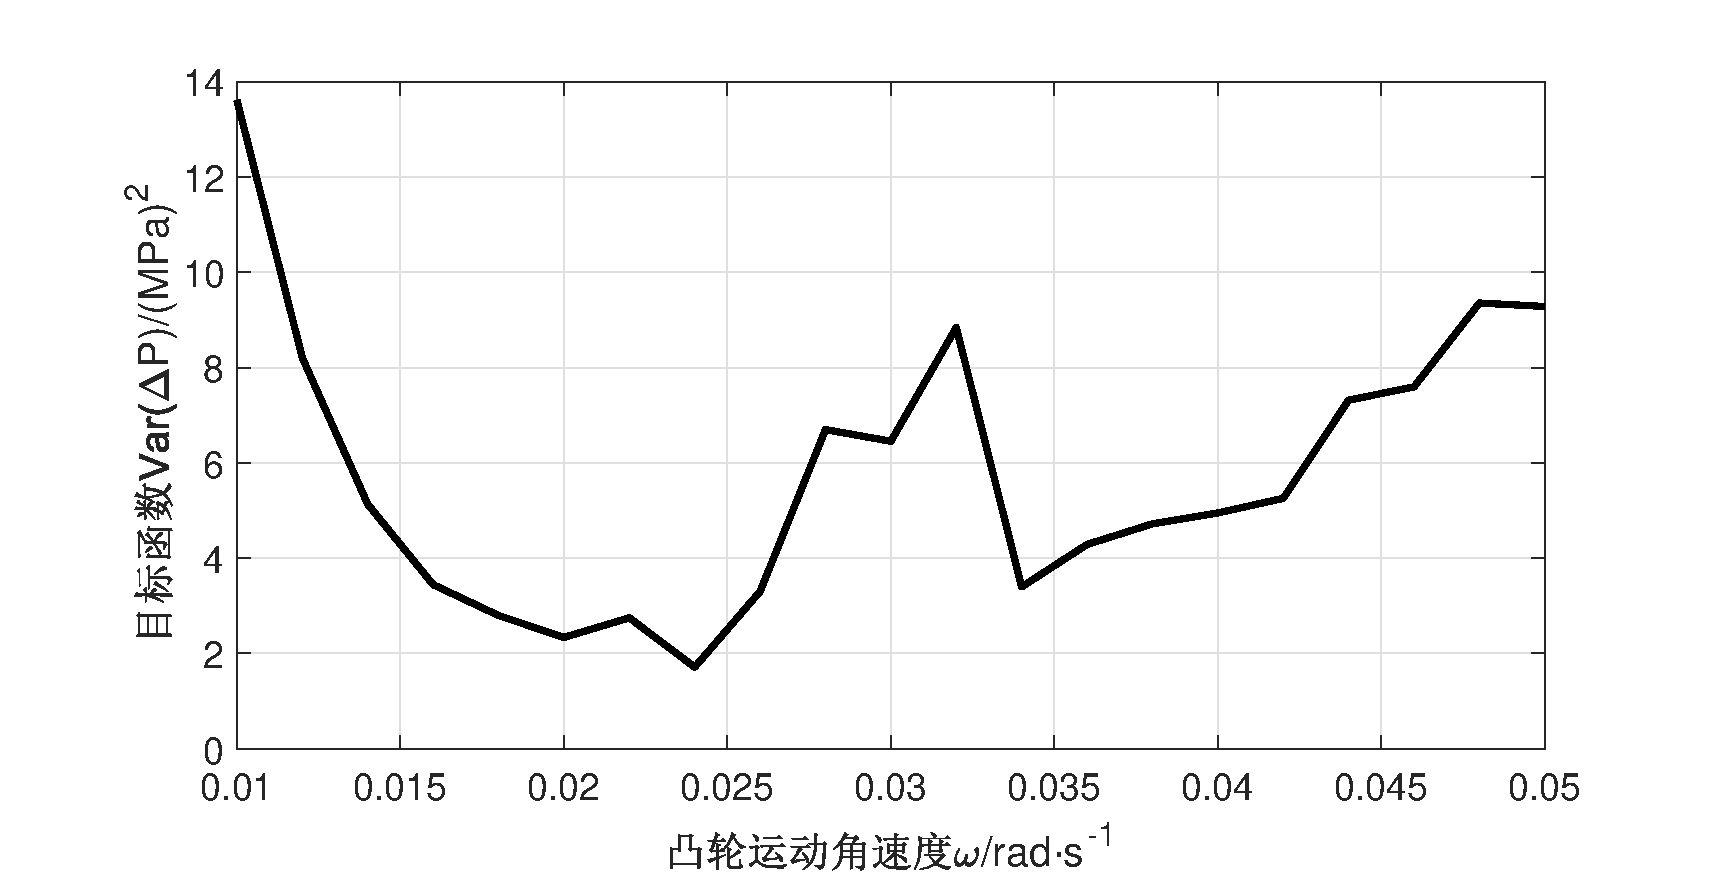
\includegraphics[scale=0.5]{Problem_2.eps}
\caption{目标函数 $\text{Var}(\Delta P)$ 与决策变量 $\omega$ 关系图}\label{Problem_2}
\end{figure}

\subsection{问题3第一问求解:双喷油器情况}
问题3第一问在问题2的基础上仅仅增加一个工作规律相同的喷油器,因此只需将原有连续性方程中的 $F_{\text{out}}$ 换为 $2F_{\text{out}}$
\begin{equation}
\label{cntequ3}
\frac{\text{d}(\Delta m)}{\text{d}t}=F_{\text{in}}-2F_{\text{out}}
\end{equation}
重新用Runge-Kutta方法结合式(\ref{Var})解式(\ref{cntequ3})得目标函数 $\text{Var}(\Delta P)$,规划得到使管内油压稳定在 $100$ MPa 的凸轮角速度最佳值为 $\omega=0.041\text{rad}\cdot\text{ms}^{-1}$(如图\ref{Problem_3_1},MATLAB代码见附件“Problem\_3\_1.m”)。
\begin{figure}[h]
\centering
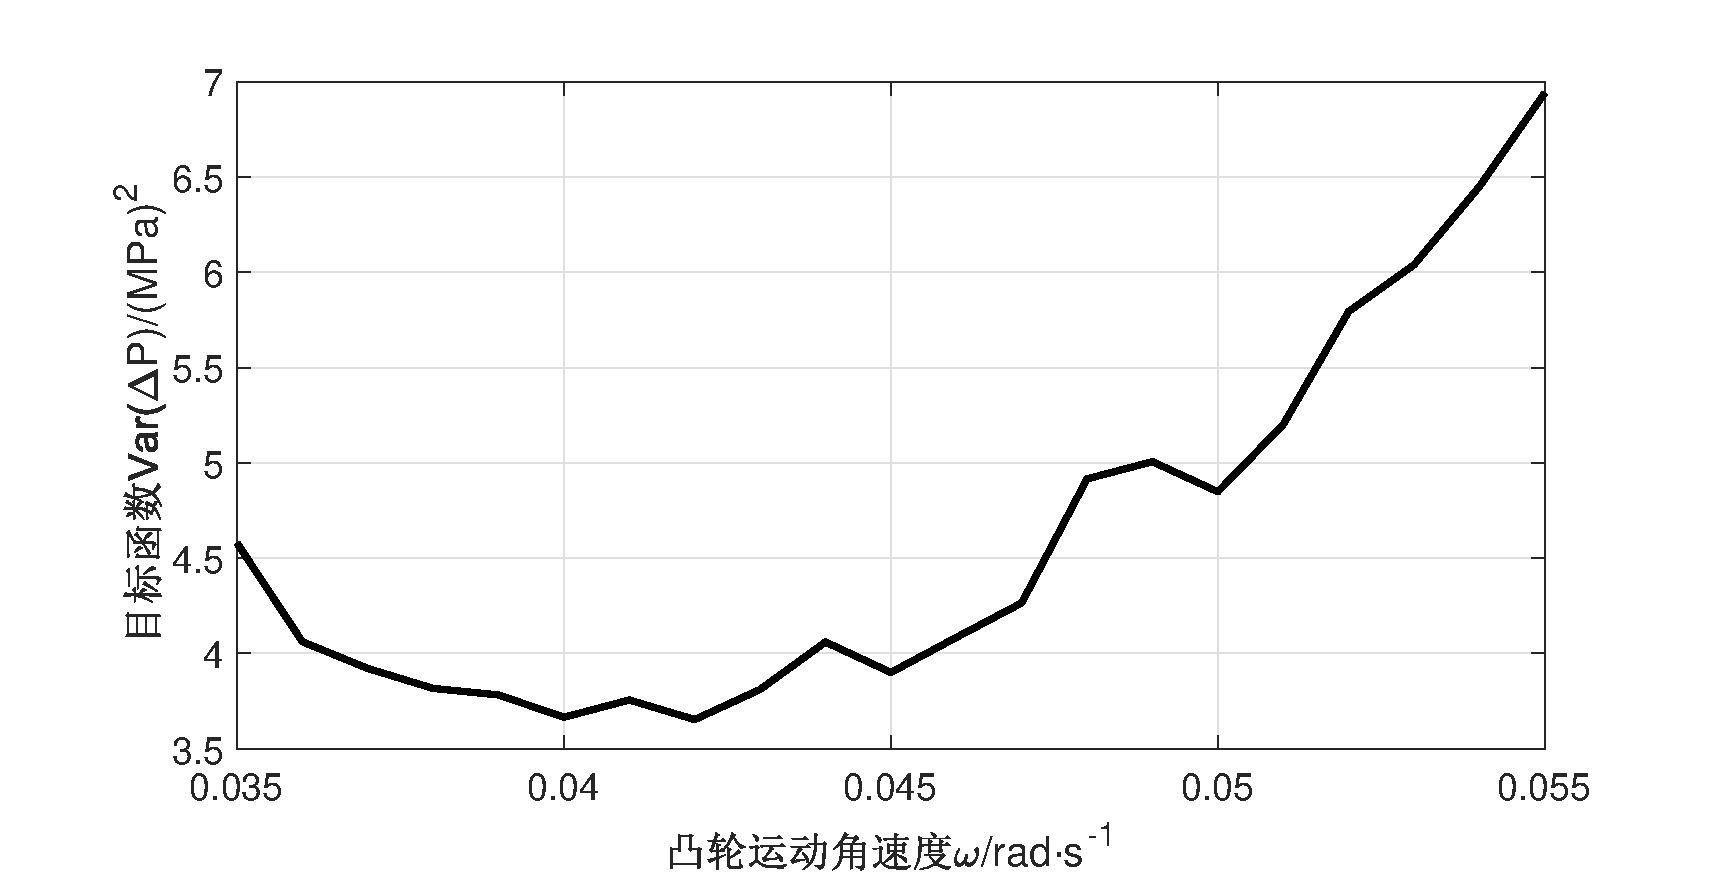
\includegraphics[scale=0.5]{Problem_3_1.eps}
\caption{目标函数 $\text{Var}(\Delta P)$ 与决策变量 $\omega$ 关系图}\label{Problem_3_1}
\end{figure}

\subsection{问题3第二问求解:双喷油器 $+$ 减压阀情况}
问题3第二问在第一问的基础上增加一个联通到外部低压油路($0.5$ MPa)中的减压阀,因此连续性方程中离开高压油管的燃油流量公式变为
\begin{equation}
\label{Foutnew}
F'_{\text{out}}=2F_{\text{out}}+F_{\text{out}2}
\end{equation}
其中 $F_{\text{out}2}$ 为单位时间内从减压阀流出高压油管的燃油质量,其可以写为
\begin{equation}
\label{Fout2}
F_{\text{out}2}=\rho Q_{\text{out}2}
\end{equation}
其中 $Q_{\text{out}2}$ 为单位时间内流出油管的燃油体积,由于减压阀的开闭由待定的压力阈值 $P_{t}$决定,只有在管内油压高于压力阈值时,减压阀才会打开,因此 $Q_{\text{out}2}$ 可以写为
\begin{equation}
\label{Qout2}
Q_{\text{out}2}=CA_{\text{out}2}\sqrt{\frac{2(P-0.5)}{\rho}}u(P-P_t)
\end{equation}
其中 $P_t$ 为减压阀开启的压强阈值。

将式(\ref{Foutnew})(\ref{Fout2})(\ref{Qout2})代入连续性方程
\begin{equation}
\frac{\text{d}(\Delta m)}{\text{d}t}=F_{\text{in}}-2F'_{\text{out}}
\end{equation}
中,根据题设保持 $\omega$ 同上小结不变,用四阶Runge-Kutta方法结合式(\ref{Var})求解得到目标函数 $\text{Var}(\Delta P)$,以减压阀开启压强阈值 $P_t$ 为决策变量,规划得其最佳值为 $P_t=102$ MPa(如图\ref{Problem_3_2},MATLAB代码见“Problem\_3\_2.m”)。
\begin{figure}[h]
\centering
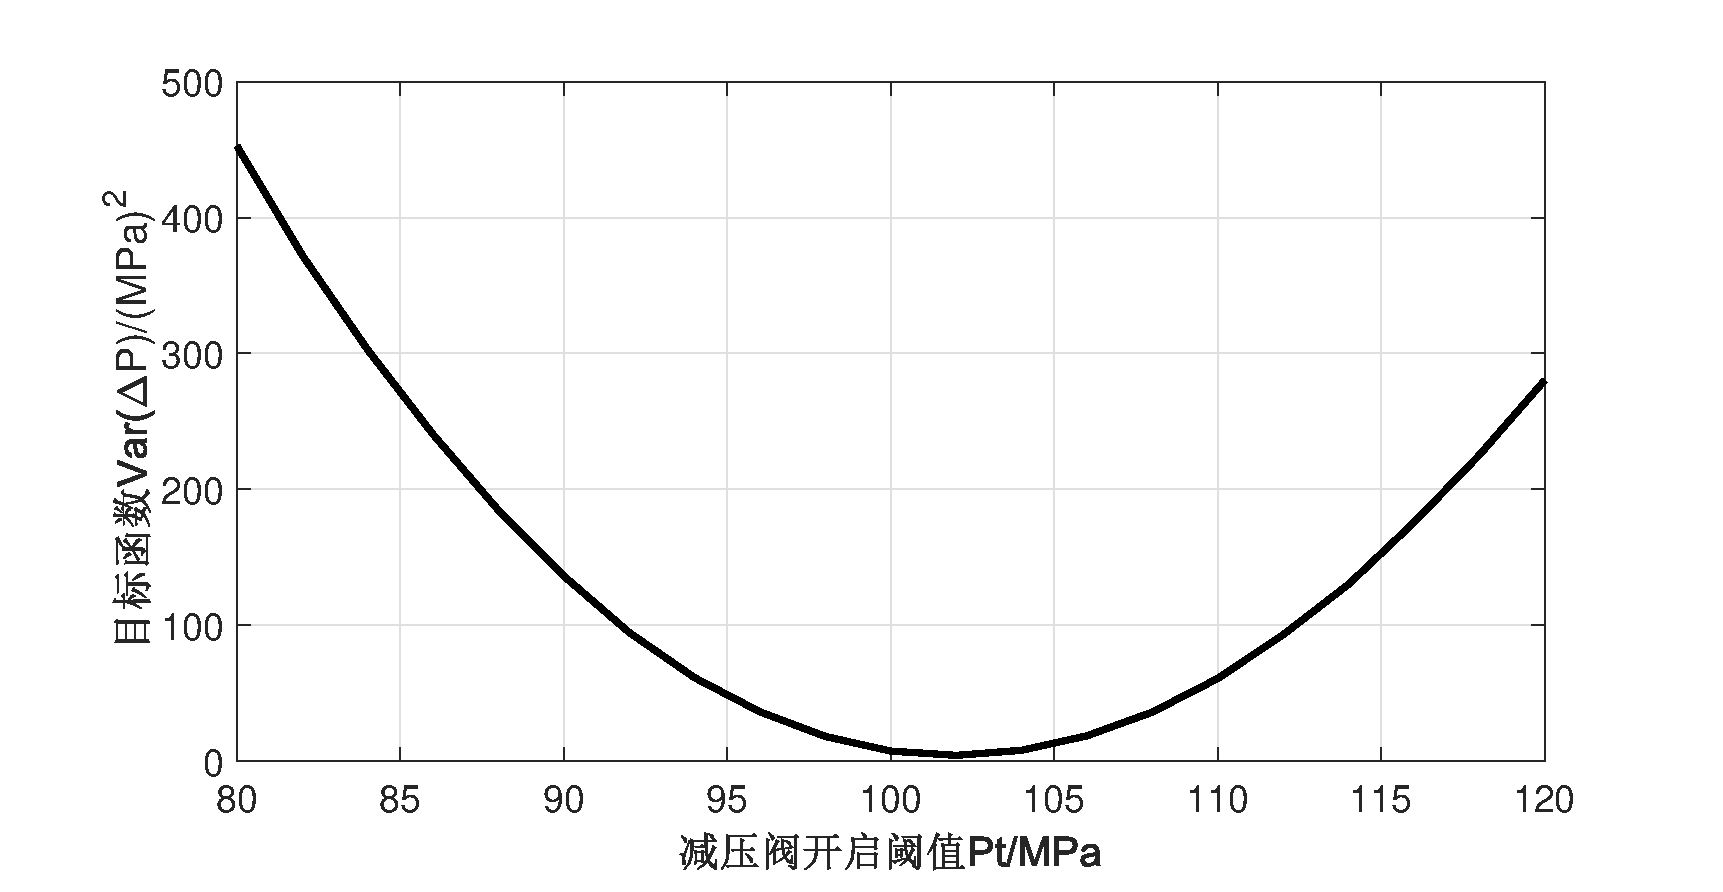
\includegraphics[scale=0.5]{Problem_3_2.eps}
\caption{目标函数 $\text{Var}(\Delta P)$ 与决策变量 $P_t$ 关系图}\label{Problem_3_2}
\end{figure}

\section{讨论和分析}

\subsection{对于问题1第二问中单向阀每次开启时长策略的讨论}
问题1第二问中单向阀每次开启时长函数还可以设为
\begin{equation}
t_0=(1-\frac{P}{150})t_{02}+\frac{P}{150}\times0.752
\end{equation}
这样可以将问题简化为单决策变量($t_{02}$)的规划问题。但考虑到实际工业应用中,单向阀的控制可能无法如上式那样平滑,因此采用原模型中的开启时长函数可能更符合实际。

\subsection{关于油管内燃油由于流速和重力产生的压强不均匀的讨论}
根据流体力学相关规律,在一定条件下,流体流速越大,则压强越小,同时重力也会影响流体的压强(在本问题中油管上下的最大压强为 $\rho gh$,大约为$10^{-8}$ MPa 量级),因此管内燃油压强并非完全均匀,本模型中忽略各局部压强差异,可能会造成一定误差。


\end{document}